\documentclass[11pt,a4paper]{ctexart}
% Shared preamble for the assignment reports. Use with:
%   \documentclass[11pt,a4paper]{ctexart}  (XeLaTeX)
%   % Shared preamble for the assignment reports. Use with:
%   \documentclass[11pt,a4paper]{ctexart}  (XeLaTeX)
%   % Shared preamble for the assignment reports. Use with:
%   \documentclass[11pt,a4paper]{ctexart}  (XeLaTeX)
%   \input{../common/preamble.tex}
\usepackage[margin=2.3cm]{geometry}
\setmainfont{texgyretermes}[Extension=.otf,UprightFont=*-regular,BoldFont=*-bold,ItalicFont=*-italic,BoldItalicFont=*-bolditalic]
\setsansfont{texgyreheros}[Extension=.otf,UprightFont=*-regular,BoldFont=*-bold,ItalicFont=*-italic,BoldItalicFont=*-bolditalic]
\setmonofont{texgyrecursor}[Extension=.otf,UprightFont=*-regular,BoldFont=*-bold,ItalicFont=*-italic,BoldItalicFont=*-bolditalic]
\usepackage{amsmath,amssymb,mathtools,bm}
\usepackage{graphicx}
\usepackage{booktabs,multirow,makecell,array,tabularx}
\usepackage[table]{xcolor}
\usepackage[most]{tcolorbox}
\usepackage{enumitem}
\usepackage{listings}
\usepackage{subcaption}
\usepackage{siunitx}
\usepackage[hidelinks]{hyperref}
\usepackage[nameinlink,noabbrev]{cleveref}
\usepackage{float}

\setlength{\emergencystretch}{3em}
\linespread{1.15}
\setlist{leftmargin=*,itemsep=2pt,topsep=3pt}
\graphicspath{{figures/}}

\crefname{figure}{图}{图}
\crefname{table}{表}{表}
\crefname{section}{第}{第}
\creflabelformat{section}{#2#1#3 节}
\crefname{equation}{式}{式}
\crefformat{equation}{式~(#2#1#3)}

\lstset{basicstyle=\ttfamily\footnotesize,columns=fullflexible,breaklines=true,frame=single,
  framerule=0.3pt,rulecolor=\color{black!40},backgroundcolor=\color{black!3},
  keywordstyle=\color{blue!60!black}\bfseries,commentstyle=\color{green!40!black},
  numbers=left,numberstyle=\tiny\color{black!50},xleftmargin=1.5em}

% Interview boxes: question, model answer, common wrong answer.
\newtcolorbox{iqbox}[1]{enhanced,breakable,colback=blue!3,colframe=blue!45!black,boxrule=0.5pt,arc=1.5pt,
  left=4pt,right=4pt,top=3pt,bottom=3pt,fonttitle=\bfseries\small,title={面试追问：#1}}
\newtcolorbox{findingbox}[1][]{enhanced,breakable,colback=green!3,colframe=green!40!black,boxrule=0.5pt,arc=1.5pt,
  left=4pt,right=4pt,top=3pt,bottom=3pt,fonttitle=\bfseries\small,title={结论#1}}
\newtcolorbox{caveatbox}{enhanced,breakable,colback=orange!4,colframe=orange!60!black,boxrule=0.5pt,arc=1.5pt,
  left=4pt,right=4pt,top=3pt,bottom=3pt,fonttitle=\bfseries\small,title={不能推出的结论}}

\newcommand{\authorline}{ShaneLiu04\thanks{GitHub: \url{https://github.com/ShaneLiu04}。代码与原始指标见 edge-deploy 仓库各 lab 的 \texttt{artifacts/raw/}。本文基于公开课程材料独立完成，与课程团队无隶属关系。}}

\usepackage[margin=2.3cm]{geometry}
\setmainfont{texgyretermes}[Extension=.otf,UprightFont=*-regular,BoldFont=*-bold,ItalicFont=*-italic,BoldItalicFont=*-bolditalic]
\setsansfont{texgyreheros}[Extension=.otf,UprightFont=*-regular,BoldFont=*-bold,ItalicFont=*-italic,BoldItalicFont=*-bolditalic]
\setmonofont{texgyrecursor}[Extension=.otf,UprightFont=*-regular,BoldFont=*-bold,ItalicFont=*-italic,BoldItalicFont=*-bolditalic]
\usepackage{amsmath,amssymb,mathtools,bm}
\usepackage{graphicx}
\usepackage{booktabs,multirow,makecell,array,tabularx}
\usepackage[table]{xcolor}
\usepackage[most]{tcolorbox}
\usepackage{enumitem}
\usepackage{listings}
\usepackage{subcaption}
\usepackage{siunitx}
\usepackage[hidelinks]{hyperref}
\usepackage[nameinlink,noabbrev]{cleveref}
\usepackage{float}

\setlength{\emergencystretch}{3em}
\linespread{1.15}
\setlist{leftmargin=*,itemsep=2pt,topsep=3pt}
\graphicspath{{figures/}}

\crefname{figure}{图}{图}
\crefname{table}{表}{表}
\crefname{section}{第}{第}
\creflabelformat{section}{#2#1#3 节}
\crefname{equation}{式}{式}
\crefformat{equation}{式~(#2#1#3)}

\lstset{basicstyle=\ttfamily\footnotesize,columns=fullflexible,breaklines=true,frame=single,
  framerule=0.3pt,rulecolor=\color{black!40},backgroundcolor=\color{black!3},
  keywordstyle=\color{blue!60!black}\bfseries,commentstyle=\color{green!40!black},
  numbers=left,numberstyle=\tiny\color{black!50},xleftmargin=1.5em}

% Interview boxes: question, model answer, common wrong answer.
\newtcolorbox{iqbox}[1]{enhanced,breakable,colback=blue!3,colframe=blue!45!black,boxrule=0.5pt,arc=1.5pt,
  left=4pt,right=4pt,top=3pt,bottom=3pt,fonttitle=\bfseries\small,title={面试追问：#1}}
\newtcolorbox{findingbox}[1][]{enhanced,breakable,colback=green!3,colframe=green!40!black,boxrule=0.5pt,arc=1.5pt,
  left=4pt,right=4pt,top=3pt,bottom=3pt,fonttitle=\bfseries\small,title={结论#1}}
\newtcolorbox{caveatbox}{enhanced,breakable,colback=orange!4,colframe=orange!60!black,boxrule=0.5pt,arc=1.5pt,
  left=4pt,right=4pt,top=3pt,bottom=3pt,fonttitle=\bfseries\small,title={不能推出的结论}}

\newcommand{\authorline}{ShaneLiu04\thanks{GitHub: \url{https://github.com/ShaneLiu04}。代码与原始指标见 edge-deploy 仓库各 lab 的 \texttt{artifacts/raw/}。本文基于公开课程材料独立完成，与课程团队无隶属关系。}}

\usepackage[margin=2.3cm]{geometry}
\setmainfont{texgyretermes}[Extension=.otf,UprightFont=*-regular,BoldFont=*-bold,ItalicFont=*-italic,BoldItalicFont=*-bolditalic]
\setsansfont{texgyreheros}[Extension=.otf,UprightFont=*-regular,BoldFont=*-bold,ItalicFont=*-italic,BoldItalicFont=*-bolditalic]
\setmonofont{texgyrecursor}[Extension=.otf,UprightFont=*-regular,BoldFont=*-bold,ItalicFont=*-italic,BoldItalicFont=*-bolditalic]
\usepackage{amsmath,amssymb,mathtools,bm}
\usepackage{graphicx}
\usepackage{booktabs,multirow,makecell,array,tabularx}
\usepackage[table]{xcolor}
\usepackage[most]{tcolorbox}
\usepackage{enumitem}
\usepackage{listings}
\usepackage{subcaption}
\usepackage{siunitx}
\usepackage[hidelinks]{hyperref}
\usepackage[nameinlink,noabbrev]{cleveref}
\usepackage{float}

\setlength{\emergencystretch}{3em}
\linespread{1.15}
\setlist{leftmargin=*,itemsep=2pt,topsep=3pt}
\graphicspath{{figures/}}

\crefname{figure}{图}{图}
\crefname{table}{表}{表}
\crefname{section}{第}{第}
\creflabelformat{section}{#2#1#3 节}
\crefname{equation}{式}{式}
\crefformat{equation}{式~(#2#1#3)}

\lstset{basicstyle=\ttfamily\footnotesize,columns=fullflexible,breaklines=true,frame=single,
  framerule=0.3pt,rulecolor=\color{black!40},backgroundcolor=\color{black!3},
  keywordstyle=\color{blue!60!black}\bfseries,commentstyle=\color{green!40!black},
  numbers=left,numberstyle=\tiny\color{black!50},xleftmargin=1.5em}

% Interview boxes: question, model answer, common wrong answer.
\newtcolorbox{iqbox}[1]{enhanced,breakable,colback=blue!3,colframe=blue!45!black,boxrule=0.5pt,arc=1.5pt,
  left=4pt,right=4pt,top=3pt,bottom=3pt,fonttitle=\bfseries\small,title={面试追问：#1}}
\newtcolorbox{findingbox}[1][]{enhanced,breakable,colback=green!3,colframe=green!40!black,boxrule=0.5pt,arc=1.5pt,
  left=4pt,right=4pt,top=3pt,bottom=3pt,fonttitle=\bfseries\small,title={结论#1}}
\newtcolorbox{caveatbox}{enhanced,breakable,colback=orange!4,colframe=orange!60!black,boxrule=0.5pt,arc=1.5pt,
  left=4pt,right=4pt,top=3pt,bottom=3pt,fonttitle=\bfseries\small,title={不能推出的结论}}

\newcommand{\authorline}{ShaneLiu04\thanks{GitHub: \url{https://github.com/ShaneLiu04}。代码与原始指标见 edge-deploy 仓库各 lab 的 \texttt{artifacts/raw/}。本文基于公开课程材料独立完成，与课程团队无隶属关系。}}

\graphicspath{{../../solutions/edge-runtime/int8-kernels/artifacts/figures/}}

\title{int8 内核实验报告：\\整数契约、requant 的两次舍入、VNNI 打包与 AMX tile}
\author{\authorline}
\date{2026 年 11 月}

\begin{document}
\maketitle

\begin{abstract}
MIT 6.5940 Lab 2 停在“模拟量化”：在 float 里乘 scale、舍入、再乘回去。端侧 runtime 真正执行的是 int8 $\times$ int8 $\to$ int32 累加，
再用一个定点乘数把 int32 requant 回 uint8。本报告把这条链路完整写了一遍——Python 参考、C++ kernel、ONNX Runtime 的 \texttt{QLinearConv} 三方逐元素比对——
再在 6 个 GEMM 形状上比较 7 种 int8 实现与 fp32，并把同一份代码搬到 Xeon Platinum 8470Q 上加测 AMX tile。
平台是一台 4 核 Ice Lake 虚拟机（AVX-512 + VNNI）和一台 Sapphire Rapids 服务器。

主要结论：
（a）int32 累加逐位精确：6 种层的累加 C++ 与 Python 参考 100\% 相等，实测 $|acc|$ 比满幅上界小 5--49 倍；
（b）TFLite 式两步定点舍入与 ORT 在 99.93--99.97\% 的输出上一致，其余永远只差 1 个量化级；不一致率按 $2^{-(\mathrm{shift}+1)}$ 变化，
    单次舍入（float 乘数或单步定点）在普通数据上与 ORT 100\% 一致；
（c）AVX2 \texttt{vpmaddubsw} 的 int16 中间和会饱和：$|w|\le 64$ 时零错误，$|w|=100$ 时 99\% 的列出错，$|w|=127$ 时全部出错；
（d）布局比指令重要：VNNI 打包 GEMM 比逐点积 VNNI 快 2.0--30.8 倍，$K=24$ 时差最大；
（e）requant 要融合：单独的标量 epilogue 把打包 GEMM 从 129 拖到 20 GOP/s，融合进寄存器后 66；
（f）ORT int8 对 fp32 在 1 线程快 1.39--3.08 倍，4 线程只有 0.76--2.14 倍，depthwise 上 int8 反而更慢；
（g）AMX 只在 $K$ 填得满 tile 时赢：$512^3$ 上 1704 GOP/s，是 VNNI 打包的 3.0 倍，LLM prefill 形状上 5.9 倍，但 $K=24$ 时只有 0.6 倍；
    GEMM 变快后单独一遍 requant 的损失从 12\% 涨到 43\%。
\end{abstract}

\tableofcontents
\newpage

\section{这个实验要回答什么}

“int8 比 fp32 快 4 倍”是面试里最常见、也最经不起追问的一句话。它隐含了三个假设：整数结果是确定的、int8 指令真能吃满、量化只是“换个数据类型”。
本实验逐条检验它们：

\begin{enumerate}
  \item \textbf{契约是否闭合？} 零点放在哪一侧、偏置用什么单位、累加器多宽、最后怎么从 int32 回到 uint8。同一组 int32 累加，
        交给 TFLite 式的定点 requant、ORT~\cite{ort} 的 float requant、精确实数 requant，结果是否逐位一致？不一致的比例能否\emph{预测}？
  \item \textbf{SIMD 指令有没有自己的契约？} AVX2 没有 u8 $\times$ s8 直接累加到 int32 的指令，\texttt{vpmaddubsw} 中间要经过饱和 int16；
        这会在什么条件下静默出错？
  \item \textbf{速度由什么决定？} 同样是 VNNI 指令，逐点积写法和 oneDNN~\cite{onednn} 式打包写法差多少？requant 这个 epilogue 放在哪里做？
        ORT 的 int8 kernel 在真实 MobileNetV2 层上对 fp32 快多少？
  \item \textbf{换到有 AMX 的服务器上结论还成立吗？} AMX 是一次吃 $16\times 64$ 字节的 tile 引擎，它对端侧模型的小通道层是否同样有效？
\end{enumerate}

前两个问题是\emph{正确性}问题，答案是确定的整数，与机器无关（\cref{sec:host} 会看到两台机器的这些指标逐位相同）；后两个是\emph{性能}问题，
答案依赖形状、编译器和硬件，本报告每一处都会给出形状与平台。服务端的 int8 GEMM 与 LLM.int8 离群值另见 mlsys-infra 的 M17 笔记；
跨主机的整体复现（屋顶~\cite{roofline}、卷积、DMA、调优、Q4 GEMV）见 edge-runtime-server 报告，本报告只深挖 int8 这一条链路，但自成一体。

\section{设置}\label{sec:setup}

\begin{table}[H]
\centering\small
\caption{平台}\label{tab:hosts}
\begin{tabularx}{\linewidth}{>{\raggedright\arraybackslash}p{2.0cm} >{\raggedright\arraybackslash}X >{\raggedright\arraybackslash}X}
\toprule
 & 本机（主实验） & 服务器（复现 + AMX） \\
\midrule
CPU & Ice Lake 服务器虚拟机（Intel64 Family 6 Model 106），4 核 / 8 线程 & 2 $\times$ Xeon Platinum 8470Q（Sapphire Rapids），绑 NUMA1 物理核 \\
ISA & AVX-512F、AVX-512 VNNI、AVX2、FMA & AVX-512、VNNI、\textbf{AMX-INT8} \\
OS / Python & Windows Server 2022，Python 3.12.10 & Linux 5.15，Python 3.12.3 \\
编译器 & MinGW g++ 13.2 & GCC 11.4 \\
ONNX Runtime & 1.31，CPUExecutionProvider & CPUExecutionProvider \\
1 线程峰值 & fp32 155 GFLOP/s，int8 396 GOP/s（host-roofline） & fp32 232 GFLOP/s，int8 617 GOP/s（host-roofline） \\
\bottomrule
\end{tabularx}
\end{table}

\begin{table}[H]
\centering\small
\caption{实验协议}\label{tab:protocol}
\begin{tabular}{lp{0.74\linewidth}}
\toprule
契约 & 激活 uint8、逐张量 scale 与零点；权重 int8 对称、逐输出通道 scale；bias int32，单位 $s_x s_w[c]$；输出 uint8（ONNX QLinearConv / TFLite 约定） \\
三方比对 & 6 种层 $\times$ 普通 / 构造 .5 平局两种输入；Python 参考（\texttt{code/int8ref/}）、C++（\texttt{cpp/int8.cpp --mode=conv}）、ORT \texttt{QLinearConv} \\
两步舍入 & 40 个对数均匀的随机乘数 $m\in[10^{-5},0.5]$，每个乘数 $10^6$ 个 $|acc|<2^{22}$ 的随机累加值，对精确舍入计不一致率 \\
饱和 & $K=256$、4096 列，激活取 128--255（类 ReLU 的大激活），权重均匀取 $[-w_{\max}, w_{\max}]$，$w_{\max}\in\{63,64,100,127\}$ \\
GEMM & 1 线程，15 次重复取中位数；权重限制在 $[-63,63]$ 使 AVX2 路径不饱和；每种 int8 实现都与标量参考逐位比对（\texttt{gemm\_all\_exact}） \\
ORT 计时 & 5 种 MobileNetV2 层，int8 \texttt{QLinearConv} 对 fp32 \texttt{Conv}，1 与 4 线程，预热 5 次后 60 次取中位数 \\
\bottomrule
\end{tabular}
\end{table}

\begin{table}[H]
\centering\small
\caption{GEMM 形状：MobileNetV2 在 $224\times224$ 输入下的 1$\times$1 卷积，$M=H\cdot W$，$K$ = 输入通道，$N$ = 输出通道}\label{tab:shapes}
\begin{tabular}{lrrrl}
\toprule
形状 & $M$ & $K$ & $N$ & 说明 \\
\midrule
pw\_expand\_56 & 3136 & 24 & 144 & 第一个 bottleneck 的 expand，$K$ 最小 \\
pw\_project\_56 & 3136 & 144 & 24 & 同一块的 project，$N$ 最小 \\
pw\_expand\_14 & 196 & 96 & 576 & 中段 expand \\
pw\_project\_14 & 196 & 576 & 96 & 中段 project，$K$ 最大的 MBv2 层 \\
pw\_head\_7 & 49 & 320 & 1280 & 分类头前的 1$\times$1 \\
square\_512 & 512 & 512 & 512 & 方阵对照 \\
llm\_prefill & 256 & 4096 & 4096 & 仅服务器：7B 注意力投影的 prefill \\
\bottomrule
\end{tabular}
\end{table}

三方比对用的 6 种层是：conv3x3\_28（$28^2$，32$\to$64）、pointwise\_28（64$\to$128）、depthwise\_28（96 通道）、
depthwise\_s2\_28（stride 2）、stem\_s2\_56（3$\to$16，stride 2）、grouped4\_28（4 组）。

\section{方法与推导}\label{sec:method}

\subsection{整数卷积与零点（E4）}

量化把实数写成 $r = s\,(q - z)$。激活 uint8 带零点 $z_x$，权重 int8 对称（$z_w = 0$），于是卷积的实数输出
\begin{equation}
y_r[c] = \sum_k s_x (x_q[k]-z_x)\cdot s_w[c]\,w_q[k,c] + b[c] = s_x s_w[c]\Big(\underbrace{\sum_k x_q[k]\,w_q[k,c] - z_x\sum_k w_q[k,c] + b_q[c]}_{acc[c]}\Big),
\label{eq:conv}
\end{equation}
其中 $b_q[c] = \mathrm{round}(b[c]/(s_x s_w[c]))$ 是 int32。这就是 E4。$z_x\sum_k w_q[k,c]$ 只依赖权重，离线折进偏置；
若权重也带零点，会多出 $-z_w\sum_k x_q[k]$ 一项，它依赖输入，每个输出位置都要再做一次归约——这就是“权重对称、激活非对称”的理由。

padding 的实数值是 0，所以 padding 位置的 uint8 值是 $z_x$，不是 0；\texttt{conv\_int32} 里直接跳过越界项，等价于 $(x-z_x)=0$。

累加器的满幅上界：激活减零点后 $|x_q - z_x|\le 255$，权重 $|w_q|\le 127$，
\begin{equation}
|acc| \le 255\cdot 127\cdot K,\qquad K = K_H K_W\cdot \mathrm{IC}/\mathrm{groups}.
\label{eq:bound}
\end{equation}
conv3x3\_28 的 $K=288$，上界 9,326,880。要触到 $2^{31}-1$ 需要 $K\ge 66{,}311$，所以对 MobileNet 一类端侧模型 int32 永远够用；
超长的全连接层或大通道 7$\times$7 卷积才需要拆部分和。

\subsection{requant 与定点乘数（E5）}

把 \cref{eq:conv} 写成输出的量化值：
\begin{equation}
y_q[c] = \mathrm{clamp}\big(z_y + \mathrm{round}(M[c]\cdot acc[c]),\,0,\,255\big),\qquad M[c] = \frac{s_x s_w[c]}{s_y} = M_0\cdot 2^{-(31+\mathrm{shift})}.
\label{eq:requant}
\end{equation}
这是 E5。逐通道量化时 $M$ 是一个长度为输出通道数的数组；ReLU / ReLU6 就是 clamp 的上下界。没有 FPU 的 MCU 上不能乘 float，
gemmlowp~\cite{jacob2018} 把 $M\in(0,1)$ 分解成 Q31 整数 $M_0\in[2^{30},2^{31})$ 和右移 $\mathrm{shift}$：\texttt{frexp} 给出 $M = q\cdot 2^{e}$、$q\in[0.5,1)$，
$M_0 = \mathrm{round}(q\cdot 2^{31})$，$\mathrm{shift} = -e$；若 $M_0$ 舍入到 $2^{31}$，减半并令 $e$ 加 1。
例：$s_x=0.02$、$s_w=0.005$、$s_y=0.05$ 时 $M=0.002=0.512\cdot 2^{-8}$，$M_0=1{,}099{,}511{,}628$，$\mathrm{shift}=8$。
$M_0$ 有 31 位精度，乘数本身的相对误差 $\le 2^{-31}$，不是输出不一致的主要来源。

\subsection{四种舍入}

本实验在 Python（\texttt{requant.py}）与 C++（\texttt{int8.cpp}）里位级一致地实现了四种 requant：

\begin{table}[H]
\centering\small
\caption{四种 requant}\label{tab:styles}
\begin{tabularx}{\linewidth}{>{\raggedright\arraybackslash}p{2.1cm} >{\raggedright\arraybackslash}p{3.4cm} >{\raggedright\arraybackslash}X >{\raggedright\arraybackslash}p{2.9cm}}
\toprule
名称 & 谁在用 & 算法 & 平局方向 \\
\midrule
fixed & TFLite / gemmlowp / CMSIS-NN & SRDHM 取 Q31 高位 + RoundingDivideByPOT，两次舍入 & SRDHM 向 $+\infty$，移位远离零 \\
fixed\_single & TFLite \texttt{TFLITE\_\allowbreak SINGLE\_\allowbreak ROUNDING} & 64 位乘积一次舍入 & 向 $+\infty$ \\
float & ORT / MLAS & fp32 乘法 + \texttt{nearbyintf} & 五成双 \\
double & 参考 & 精确实数乘法 & 远离零 \\
\bottomrule
\end{tabularx}
\end{table}

两步定点的核心是两个函数：

\begin{lstlisting}[language=C++]
static int32_t srdhm(int32_t a, int32_t b) {  // SaturatingRoundingDoublingHighMul
    if (a == b && a == INT32_MIN) return INT32_MAX;
    int64_t ab = static_cast<int64_t>(a) * b;
    int64_t nudge = ab >= 0 ? (1ll << 30) : (1 - (1ll << 30));
    return static_cast<int32_t>((ab + nudge) / (1ll << 31));
}
static int32_t rounding_divide_by_pot(int32_t x, int exponent) {
    int32_t mask = (1 << exponent) - 1;
    int32_t remainder = x & mask;
    int32_t threshold = (mask >> 1) + (x < 0 ? 1 : 0);
    return (x >> exponent) + (remainder > threshold ? 1 : 0);
}
\end{lstlisting}

SRDHM 先加 $2^{30}$ 再截断，相当于把 $acc\cdot M_0/2^{31}$ 舍入到整数；第二步再把它右移 $\mathrm{shift}$ 位并舍入。
直接用 \texttt{>>} 代替第二步是截断，会给每层带来系统性的负偏差。

\paragraph{两步舍入的不一致率（E6 前半）。} 设精确值 $v = acc\cdot M$（输出单位）。第一步得到整数 $t=\mathrm{round}(v\cdot 2^{\mathrm{shift}})$，
相当于把 $v$ 量化到 $2^{-\mathrm{shift}}$ 的网格上；第二步计算 $\mathrm{round}(t/2^{\mathrm{shift}})$。问题出在第一步\emph{制造}了平局：
当 $t \bmod 2^{\mathrm{shift}} = 2^{\mathrm{shift}-1}$ 时，$t/2^{\mathrm{shift}}$ 恰好落在 .5 上，第二步按“远离零”进位；
而原始的 $v$ 在 $[\,n+0.5-2^{-(\mathrm{shift}+1)},\, n+0.5+2^{-(\mathrm{shift}+1)})$ 里均匀分布，其中一半在 .5 以下，精确舍入应当舍去。
$v$ 的小数部分近似均匀时，$t$ 落在这个余数上的概率是 $2^{-\mathrm{shift}}$，再乘以一半：
\begin{equation}
P(\text{fixed}\neq\text{exact}) \approx \tfrac12\cdot 2^{-\mathrm{shift}} = 2^{-(\mathrm{shift}+1)}.
\label{eq:double}
\end{equation}
所以乘数越大（shift 越小）越常见；不一致永远只差 1 个级。单次舍入没有中间网格，只在 $v$ 本身是精确平局时与“远离零”不同（方向向 $+\infty$），
或者 $M_0$ 的 $2^{-31}$ 相对误差恰好把 $v$ 推过 .5，这两种事件都罕见得多。

\paragraph{float 与五成双。} ORT 用 fp32 乘 float 乘数后 \texttt{nearbyintf}：默认舍入模式下是四舍六入五成双。它与 double 参考只在精确平局上不同，
差的正好是偶数侧舍入的那一半平局。

\subsection{\texttt{vpmaddubsw} 的饱和（E6 后半）}

AVX2 的 int8 点积是两条指令：\texttt{vpmaddubsw} 把相邻两对 u8 $\times$ s8 乘积相加成\emph{饱和} int16，再用 \texttt{vpmaddwd} 乘 1 加到 int32：
\begin{equation}
x_{2i}w_{2i} + x_{2i+1}w_{2i+1} \le 2\cdot 255\cdot \max|w| \le 32767 \;\Longrightarrow\; \max|w| \le 64.
\label{eq:sat}
\end{equation}
满幅 int8 权重下这一对和可达 $2\cdot 255\cdot 127 = 64770$，会静默截到 32767。工程上的解法有三个：权重限制在 7 bit，激活限制在 7 bit，
或者换 AVX-512 VNNI——\texttt{vpdpbusd} 一条指令完成 4 对 u8 $\times$ s8 乘积并直接累加到 int32，没有 int16 中间步骤。

\subsection{VNNI 打包与寄存器块}\label{sec:pack}

朴素写法“每个输出一个点积”：沿 $K$ 用 \texttt{vpdpbusd} 累加到一个 16 lane 的 zmm，最后做一次 16 lane 的水平求和。$K$ 很小时，
一次点积只有几十个乘加，水平求和与尾部处理就占满了时间。oneDNN 式打包把权重重排成 $[N/16][K/4][16\text{ 列}][4\text{ 个 }k]$：

\begin{lstlisting}[language=C++]
static std::vector<int8_t> pack_vnni(int N, int K, const int8_t* Wnk, int kb_pad = 0) {
    int nb = (N + 15) / 16, kb = std::max(kb_pad, (K + 3) / 4);
    std::vector<int8_t> p(static_cast<size_t>(nb) * kb * 64, 0);
    for (int n = 0; n < N; ++n)
        for (int k = 0; k < K; ++k)
            p[((static_cast<size_t>(n / 16) * kb + k / 4) * 16 + n % 16) * 4 + k % 4] =
                Wnk[static_cast<size_t>(n) * K + k];
    return p;
}
\end{lstlisting}

内循环每次把 $x[k..k{+}3]$ 的 4 个字节广播成一个 32 位标量填满 zmm，乘一次 64 字节的权重加载，就同时推进 16 个输出列；
累加器沿 $N$ 方向排开，留在寄存器里，最后不需要水平求和。本实现的寄存器块是 $R\le 4$ 行 $\times$ 32 列（两个 16 列块），共 8 个 zmm 累加器；
没有更大的 M 方向寄存器分块，也没有 K / N 方向的 cache 分块，离 oneDNN / XNNPACK 还差一截。

\paragraph{AMX tile。} 服务器上的 \texttt{gemm\_u8s8\_amx} 先用 \texttt{arch\_prctl(ARCH\_REQ\_XCOMP\_PERM, XFEATURE\_XTILEDATA)} 向 Linux 申请 8 KB 的 tile 状态，
配置 8 个 16 行 $\times$ 64 字节的 tile，做 $2\times2$ 输出块：tmm0--3 累加，tmm4--5 读 A 的两个 16 行块，tmm6--7 读 B 的两个 16 列块。
一条 \texttt{\_tile\_dpbusd} 计算 $C[16\times16\ \text{int32}] \mathrel{+}= A[16\times 64\ \text{u8}]\cdot B[16\ \text{个 k-quad}\times(16\times 4)\ \text{s8}]$，
B 正好是 \texttt{pack\_vnni} 在连续 64 个 $k$ 上的一个 16 列块，所以 VNNI 打包可以直接复用；$K$ 不足 64 的倍数时在打包时补零（\texttt{kb\_pad}），
$M$ 补到 32 的倍数。tile 的 $K$ 宽度固定 64 字节，所以有效乘加比例是
\begin{equation}
\eta(K) = \frac{K}{64\lceil K/64\rceil},\qquad \eta(24) = 37.5\%,\quad \eta(96)=75\%,\quad \eta(144)=75\%,\quad \eta(512)=100\%.
\label{eq:fill}
\end{equation}

\subsection{epilogue 与 Amdahl}\label{sec:amdahl}

每个 int8 GEMM 都要一个 epilogue：加零点修正项 $-z_x\sum_k w$、乘 $M_0$、SRDHM、舍入右移、加 $z_y$、clamp。本实验比较三种放法：

\begin{itemize}
  \item \textbf{标量 epilogue}：GEMM 把 int32 累加器写回内存，再逐元素调用标量 \texttt{requant\_fixed}；
  \item \textbf{SIMD epilogue}：同样写回，再用 \texttt{requant16} 一次处理 16 列（逐列参数以 SoA 形式 \texttt{RequantSoA} 加载）；
        SRDHM 需要 32$\times$32$\to$64 位乘法，AVX-512 只有偶数 lane 的 \texttt{\_mm512\_mul\_epi32}，所以奇偶 lane 各算一次再拼回；
  \item \textbf{融合}：在 \texttt{vnni\_block} 末尾直接对寄存器里的累加器调用 \texttt{requant16}，写 uint8，int32 tile 从不落到内存。
\end{itemize}

三者与标量参考的 uint8 输出逐位相同。若单独一遍 requant 占总时间的比例为 $f$，GEMM 本身加速 $s$ 倍后整体只加速
\begin{equation}
S = \frac{1}{(1-f)/s + f},
\label{eq:amdahl}
\end{equation}
requant 的绝对时间不随 GEMM 变快而变短，所以 GEMM 越快，epilogue 的份额越大（\cref{sec:amx}）。

\section{三方比对：累加精确，舍入差 1 级}\label{sec:agree}

\begin{table}[H]
\centering\small
\caption{三方比对（\texttt{requant\_agreement.csv}）：各 requant 方式与 ORT \texttt{QLinearConv} 输出的一致率}\label{tab:agree}
\begin{tabular}{lrrrrrr}
\toprule
层 & 输出数 & max$|acc|$ & 上界 & 两步定点 & 单步定点 & float \\
\midrule
conv3x3\_28 & 50,176 & 192,519 & 9,326,880 & 99.966\% & 100\% & 100\% \\
pointwise\_28 & 100,352 & 73,160 & 2,072,640 & 99.949\% & 100\% & 100\% \\
depthwise\_28 & 75,264 & 56,310 & 291,465 & 99.928\% & 100\% & 100\% \\
depthwise\_s2\_28 & 18,816 & 50,470 & 291,465 & 99.942\% & 100\% & 100\% \\
stem\_s2\_56 & 12,544 & 65,498 & 874,395 & 99.936\% & 100\% & 100\% \\
grouped4\_28 & 50,176 & 95,615 & 4,663,440 & 99.960\% & 100\% & 100\% \\
\bottomrule
\end{tabular}
\end{table}

\begin{table}[H]
\centering\small
\caption{构造 .5 平局的同一组层：与 ORT 的一致率}\label{tab:ties}
\begin{tabular}{lrrrr}
\toprule
层 & 两步定点 & 单步定点 & float & double（远离零） \\
\midrule
conv3x3\_28 & 99.546\% & 99.870\% & 100\% & 99.713\% \\
pointwise\_28 & 99.456\% & 99.757\% & 100\% & 99.737\% \\
depthwise\_28 & 98.968\% & 99.491\% & 100\% & 99.475\% \\
depthwise\_s2\_28 & 98.985\% & 99.495\% & 100\% & 99.532\% \\
stem\_s2\_56 & 99.482\% & 99.721\% & 100\% & 99.745\% \\
grouped4\_28 & 99.550\% & 99.753\% & 100\% & 99.777\% \\
\bottomrule
\end{tabular}
\end{table}

读法：

\begin{itemize}
  \item \textbf{累加是逐位精确的。} 12 个层 / 输入组合上，C++ 的 int32 累加与 Python 参考 100\% 相等，C++ 的 fixed / float / double 三种 requant 输出也与 Python 逐位一致（\texttt{cpp\_all\_exact = true}）。
        整数运算没有“误差”，只有“规则”。
  \item \textbf{上界远未触到。} max$|acc|$ 比 \cref{eq:bound} 的上界小 5.2（depthwise\_28）到 48.8 倍（grouped4\_28）。$K=9$ 的 depthwise 最贴近上界：
        归约越短，随机符号相互抵消越少。真实数据不满幅，但上界是写 kernel 时唯一能依赖的保证。
  \item \textbf{两步定点与 ORT 差 0.03--0.07\%。} 每个不一致只差 1（\texttt{ort\_maxdiff\_fixed = 1}）。按 M02 笔记，6 层各通道的 shift 中位数是 9--11，
        \cref{eq:double} 预测 $2^{-10}$ 到 $2^{-12}$，即约 0.02\%--0.1\%，实测落在这个区间里。
  \item \textbf{平局把舍入规则暴露出来。} 构造平局后 ORT 与 float 参考仍是 100\%（两者都是五成双），与 double 参考降到 99.48--99.78\%——
        差的正是平局里偶数侧那一半；两步定点降到 98.97--99.55\%，单步定点 99.49--99.87\%（向 $+\infty$ 与五成双在负数平局上方向不同）。
\end{itemize}

\begin{findingbox}[：位级一致只在同一种舍入规则内成立]
同一组 int32 累加，交给三种 requant 规则，会在约 0.05\% 的输出上差 1 个量化级；这不是 bug，而是契约里没写死的那一行。
部署验收时，参考输出必须按目标 runtime 的舍入规则生成；跨 runtime 比对要允许 1 级差异并报告比例，比例与 $2^{-(\mathrm{shift}+1)}$ 吻合时就是契约差异。
\end{findingbox}

\section{两步舍入的不一致率}\label{sec:double}

\begin{figure}[H]
\centering
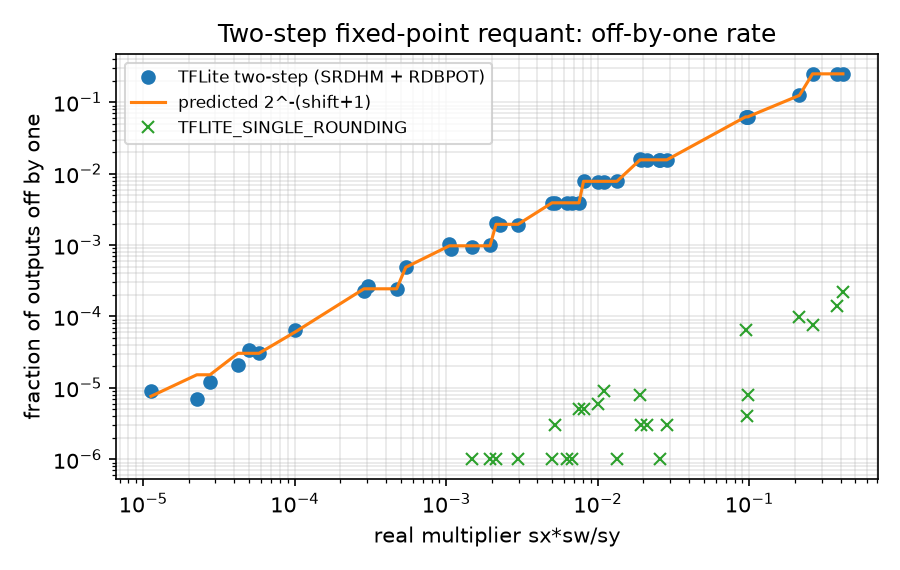
\includegraphics[width=0.82\linewidth]{double_rounding.png}
\caption{本机：两步定点 requant（SRDHM + RoundingDivideByPOT，圆点）对精确舍入的不一致率随实数乘数 $s_x s_w/s_y$ 的变化；
折线是 \cref{eq:double} 的预测 $2^{-(\mathrm{shift}+1)}$，叉号是 \texttt{TFLITE\_SINGLE\_ROUNDING}（只画出非零点）。每个乘数 $10^6$ 个累加值。}\label{fig:double}
\end{figure}

\Cref{fig:double} 是本实验最“干净”的一张图：40 个圆点几乎全贴在阶梯折线上。阶梯来自 shift 是整数——乘数每翻一倍，shift 减 1，不一致率翻一倍；
同一个 shift 内的乘数共享同一个台阶。具体数值（\texttt{double\_rounding.csv}）：

\begin{table}[H]
\centering\small
\caption{两步舍入不一致率：预测与实测（节选）}\label{tab:double}
\begin{tabular}{rrrrr}
\toprule
乘数 $m$ & shift & 预测 $2^{-(\mathrm{shift}+1)}$ & 两步定点 & 单步定点 \\
\midrule
$1.13\times10^{-5}$ & 16 & $7.6\times10^{-6}$ & $9\times10^{-6}$ & 0 \\
$2.26\times10^{-5}$ & 15 & $1.5\times10^{-5}$ & $7\times10^{-6}$ & 0 \\
$1.05\times10^{-3}$ & 9 & $9.8\times10^{-4}$ & $1.03\times10^{-3}$ & 0 \\
$2.13\times10^{-3}$ & 8 & $1.95\times10^{-3}$ & $2.01\times10^{-3}$ & $1\times10^{-6}$ \\
$1.90\times10^{-2}$ & 5 & $1.56\times10^{-2}$ & $1.58\times10^{-2}$ & $8\times10^{-6}$ \\
$9.45\times10^{-2}$ & 3 & $6.25\times10^{-2}$ & $6.18\times10^{-2}$ & $6.5\times10^{-5}$ \\
$0.415$ & 1 & $0.25$ & $0.2506$ & $2.2\times10^{-4}$ \\
\bottomrule
\end{tabular}
\end{table}

两步定点的实测 / 预测比在 0.46（shift 15）到 1.18（shift 16）之间：shift 大时 $10^6$ 个样本里只有几个到十几个不一致事件，相对波动大；
shift $\le 9$ 时事件数上千，实测与预测几乎重合（shift 1：0.2498--0.2506 对 0.25）。单步定点的不一致率在小乘数上恒为 0，
在 shift 1 时最多 $2.2\times 10^{-4}$，比两步定点低三个数量级以上；这部分来自精确平局的方向（向 $+\infty$ 对远离零）和 $M_0$ 的 Q31 截断误差，
不再随 shift 指数变化。

这张图同时解释了两个工程现象。第一，端侧模型里 $M = s_x s_w/s_y$ 常见在 $10^{-3}$ 量级（shift 约 9），不一致率约 0.1\%，与 \cref{tab:agree} 吻合；
但若某层输出 scale 很小、乘数接近 0.5，不一致率可以到 25\%——此时 TFLite 与 ORT 的输出看起来“差很多”，其实仍然只是 1 级的舍入差。
第二，消除它的办法不是换 float，而是一次舍入：TFLite 的 \texttt{TFLITE\_SINGLE\_ROUNDING} 需要一次 32$\times$32$\to$64 位乘法，Cortex-M 上有 \texttt{SMULL}，开销很小。

\begin{iqbox}{为什么 requant 要用定点，而不是直接乘一个 float？}
Cortex-M0 / M3 没有 FPU，float 乘法要软件模拟；有 FPU 的芯片上，float 结果还会受编译选项影响（FMA 收缩、舍入模式），不能保证位级可复现。
定点 $M_0\cdot 2^{-(31+\mathrm{shift})}$ 在任何平台上结果都相同——本实验两台机器、两种编译器（GCC 13.2 / 11.4）的不一致率表逐位相同（\cref{sec:host}）。
代价是两步舍入在约 $2^{-(\mathrm{shift}+1)}$ 的输出上与精确舍入差 1 级；需要和 float 路径完全对齐时用单步舍入。
\end{iqbox}

\section{\texttt{vpmaddubsw} 的饱和}\label{sec:sat}

\begin{table}[H]
\centering\small
\caption{\texttt{maddubs\_saturation.csv}：$K=256$、4096 列，AVX2 \texttt{vpmaddubsw} 路径对标量参考}\label{tab:sat}
\begin{tabular}{rrrrrr}
\toprule
 & \multicolumn{2}{c}{本机（Ice Lake）} & \multicolumn{2}{c}{服务器（8470Q）} & \\
\cmidrule(lr){2-3}\cmidrule(lr){4-5}
max$|w|$ & 出错列 & 最大绝对误差 & 出错列 & 最大绝对误差 & $2\cdot255\cdot\max|w|$ \\
\midrule
63 & 0 & 0 & 0 & 0 & 32,130 \\
64 & 0 & 0 & 0 & 0 & 32,640 \\
100 & 4053（99.0\%） & 43,326 & 4017（98.1\%） & 35,867 & 51,000 \\
127 & 4096（100\%） & 111,688 & 4096（100\%） & 118,434 & 64,770 \\
\bottomrule
\end{tabular}
\end{table}

阈值与 \cref{eq:sat} 完全吻合：$w_{\max}=64$ 时最坏一对和 32,640 $<$ 32,767，零错误；$w_{\max}=100$ 时激活取 128--255（ReLU 之后的大激活），
4096 列里 98--99\% 至少有一对饱和，一列的误差累积到 3.6--4.3 万，相当于把一个 int32 累加值整体拉偏；$w_{\max}=127$ 时每一列都错。
两台机器的出错列数略有不同（4053 对 4017），因为随机数来自 C 库的 \texttt{std::rand}，MinGW 与 glibc 的序列不同；阈值完全相同。

这个错误是\emph{静默}的：结果仍然是合法的 int32，测试数据不满幅时根本发现不了。所以 AVX2 int8 路径要么把权重限制在 7 bit，
要么像 oneDNN 那样在无 VNNI 的机器上把权重缩放 0.5、在 requant 里补偿。VNNI 的 \texttt{vpdpbusd} 直接累加到 int32，没有这个问题；
本实验的 GEMM 计时把权重限制在 $[-63,63]$，正是为了让 AVX2 路径在计时时也是正确的。

\begin{iqbox}{AVX2 上权重最大到 80，用 \texttt{vpmaddubsw} 安全吗？}
不安全：$2\cdot255\cdot80 = 40{,}800 > 32{,}767$。是否真的出错取决于激活分布——激活小时可能侥幸不饱和，ReLU 后的大激活一定会触发。
本实验 $|w|=100$、激活 128--255 时 99\% 的列出错。可选方案：量化时把权重截到 $[-64,64]$（精度损失约 1 bit），或者激活用 7 bit，
或者改用 \texttt{vpmaddwd} 的 16 位路径（吞吐减半），有 VNNI 就用 \texttt{vpdpbusd}。
\end{iqbox}

\section{GEMM：7 种 int8 实现对 fp32}\label{sec:gemm}

\begin{figure}[H]
\centering
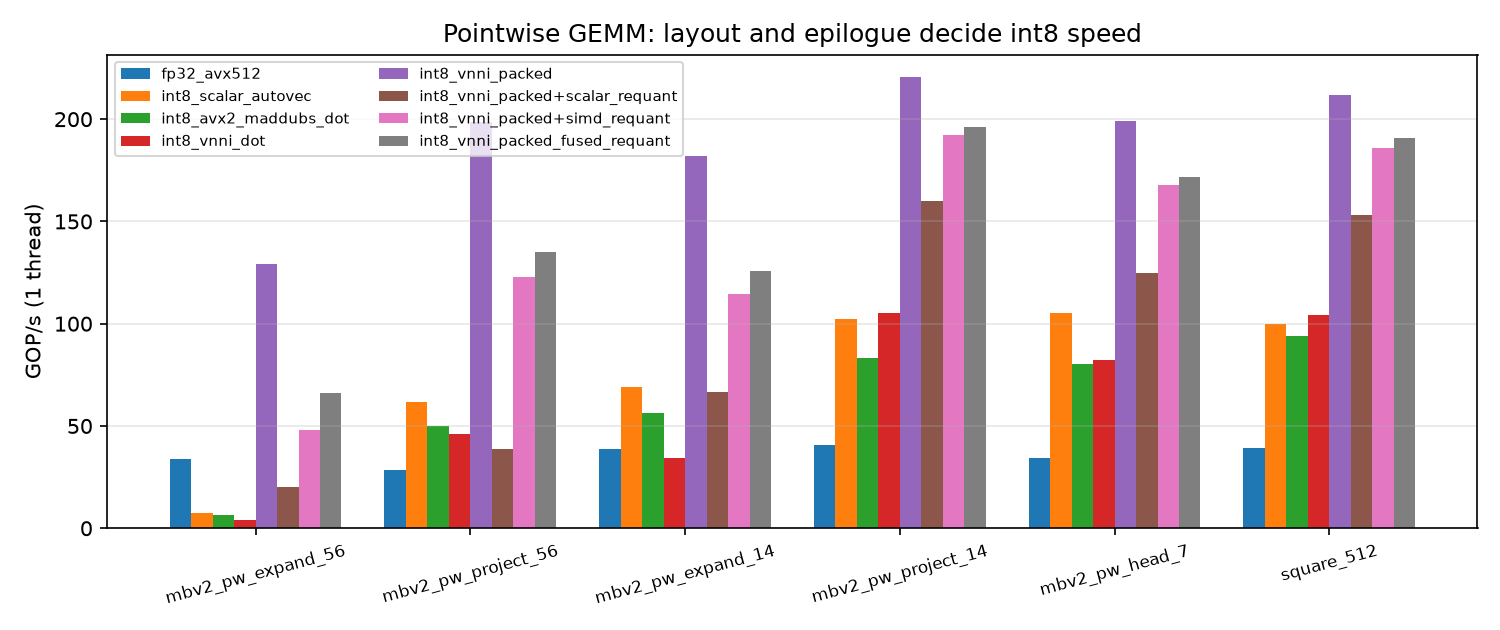
\includegraphics[width=\linewidth]{gemm_bench.png}
\caption{本机 1 线程 GEMM 吞吐（GOP/s，一次乘加计 2 次运算）。每组柱从左到右：fp32 AVX-512、int8 标量（编译器自动向量化）、AVX2 maddubs 逐点积、
VNNI 逐点积、VNNI 打包、打包 + 标量 requant、打包 + SIMD requant、打包 + 融合 requant。}\label{fig:gemm}
\end{figure}

\begin{table}[H]
\centering\small
\caption{本机 1 线程 GOP/s（\texttt{summary.json}）。所有 int8 输出与参考逐位相等（\texttt{gemm\_all\_exact}）}\label{tab:gemm}
\setlength{\tabcolsep}{4pt}
\begin{tabular}{lrrrrrrrr}
\toprule
形状 & fp32 & 标量 & maddubs & VNNI 点积 & VNNI 打包 & + 标量 rq & + SIMD rq & 融合 rq \\
\midrule
pw\_expand\_56 & 33.8 & 7.5 & 6.3 & 4.2 & 129.0 & 20.2 & 48.1 & 66.0 \\
pw\_project\_56 & 28.3 & 61.7 & 50.2 & 46.2 & 198.6 & 38.9 & 122.8 & 135.3 \\
pw\_expand\_14 & 38.7 & 68.9 & 56.2 & 34.1 & 182.0 & 66.6 & 114.6 & 125.6 \\
pw\_project\_14 & 40.6 & 102.4 & 83.0 & 105.2 & 220.6 & 160.0 & 192.4 & 196.4 \\
pw\_head\_7 & 34.3 & 105.0 & 80.4 & 82.4 & 199.0 & 125.0 & 167.6 & 171.9 \\
square\_512 & 39.2 & 99.8 & 94.2 & 104.4 & 211.8 & 153.0 & 185.8 & 190.8 \\
\bottomrule
\end{tabular}
\end{table}

\begin{table}[H]
\centering\small
\caption{由 \cref{tab:gemm} 算出的比值}\label{tab:gemmratio}
\begin{tabular}{lrrrrr}
\toprule
形状 & $K$ & 打包 / VNNI 点积 & 打包 / fp32 & 融合 / 标量 rq & SIMD rq 损失 \\
\midrule
pw\_expand\_56 & 24 & 30.8 & 3.8 & 3.3 & 63\% \\
pw\_project\_56 & 144 & 4.3 & 7.0 & 3.5 & 38\% \\
pw\_expand\_14 & 96 & 5.3 & 4.7 & 1.9 & 37\% \\
pw\_project\_14 & 576 & 2.1 & 5.4 & 1.2 & 13\% \\
pw\_head\_7 & 320 & 2.4 & 5.8 & 1.4 & 16\% \\
square\_512 & 512 & 2.0 & 5.4 & 1.2 & 12\% \\
\bottomrule
\end{tabular}
\end{table}

\Cref{fig:gemm} 里最显眼的是紫色柱（VNNI 打包）：它在每个形状上都是最高的一根，比同样用 \texttt{vpdpbusd} 的红色柱（逐点积）高一大截。按形状读：

\begin{itemize}
  \item \textbf{同一条指令，布局差 2.0--30.8 倍。} 逐点积的每个输出都要一次 16 lane 水平求和；$K=24$ 时一次点积只有 24 个乘加，连一个 64 字节向量都填不满，
        水平求和与尾部处理占满时间，所以 VNNI 点积（4.2）比编译器自动向量化的标量（7.5）还慢。打包后输出沿 $N$ 方向 16 个一组，累加器留在寄存器，
        没有水平求和，同一形状 129 GOP/s。$K\ge 512$ 时一次点积够长，水平求和被摊薄，差距收敛到 2 倍左右。
  \item \textbf{AVX2 maddubs 不比标量快。} 编译器（GCC 13.2）已经把标量 int8 循环自动向量化成 VNNI（\cref{sec:host} 有汇编证据），
        手写的 maddubs 路径多一条 \texttt{vpmaddwd}，在每个形状上都比“标量”慢 6--23\%。
  \item \textbf{打包 GEMM 最高 221 GOP/s，是本机实测 int8 峰值 396 的 56\%。} 对 fp32 的 5.4 倍（square\_512）高于“int8 峰值 / fp32 峰值”= 396/155 = 2.56，
        因为本实验的 fp32 GEMM 本身只到峰值的约四分之一（39 对 155），不是一个调优过的基线；所以“int8 比 fp32 快几倍”取决于 fp32 基线有多好，
        \cref{sec:ort} 里 ORT 的对比更公平。
  \item \textbf{requant 的代价与 $K$ 成反比。} epilogue 的工作量是 $M\times N$，GEMM 是 $M\times N\times K$。$K=24$ 时标量 requant 把 129 拖到 20（慢 6.4 倍），
        $K=576$ 时只从 221 到 160（慢 1.4 倍）。SIMD epilogue 把 $K=24$ 的损失从 84\% 降到 63\%，融合再降到 49\%（66.0 对 129.0）。
  \item \textbf{融合不是免费的。} 即使不写回 int32，requant 的算术本身（奇偶 lane 两次 64 位乘、移位、比较、clamp）仍要花指令：
        square\_512 上融合版 190.8 比纯 GEMM 211.8 低 10\%。融合省掉的是内存往返——int32 累加器是 uint8 输出的 4 倍字节——不是计算。
\end{itemize}

\begin{findingbox}[：布局与 epilogue 比指令重要]
在小通道的端侧层上，决定 int8 速度的不是“有没有 VNNI”，而是\emph{累加器在哪里}：逐点积把累加器摊在 lane 上、最后水平求和，打包把累加器沿输出列排开、
留在寄存器。同一条 \texttt{vpdpbusd}，$K=24$ 时两种写法差 30.8 倍。打包之后的瓶颈转到 epilogue：$K=24$ 的层上单独一遍标量 requant 吃掉 84\% 的吞吐，
融合进寄存器后比标量 epilogue 快 1.2--3.5 倍。
\end{findingbox}

\begin{iqbox}{int8 GEMM 的 requant 放在哪里做？为什么？}
融合进 GEMM 的寄存器阶段：累加完一个 $R\times 32$ 的块后，直接在 zmm 里加零点修正、乘 $M_0$、SRDHM、舍入右移、加 $z_y$、clamp，写 uint8。
这样 int32 tile（输出字节的 4 倍）从不落到内存。本机 pw\_expand\_56（$K=24$）上，单独标量 epilogue 把 129 GOP/s 拖到 20，融合后 66；
$K$ 越小，GEMM 每个输出做的乘加越少，epilogue 占比越大，融合越重要。逐通道量化不改变累加，只是 epilogue 的参数从标量变成按列加载的数组（SoA）。
\end{iqbox}

\section{ONNX Runtime：int8 \texttt{QLinearConv} 对 fp32 \texttt{Conv}}\label{sec:ort}

\begin{table}[H]
\centering\small
\caption{本机 ORT 1.31，单层中位数（$\mu$s），\texttt{ort\_int8\_vs\_fp32.csv}}\label{tab:ort}
\begin{tabular}{lrrrrrr}
\toprule
层 & 1 线程 fp32 & 1 线程 int8 & 加速 & 4 线程 fp32 & 4 线程 int8 & 加速 \\
\midrule
pw\_expand\_56 & 426 & 230 & 1.86 & 333 & 156 & 2.14 \\
pw\_project\_56 & 453 & 155 & 2.92 & 257 & 151 & 1.70 \\
pw\_expand\_14 & 219 & 88 & 2.49 & 124 & 100 & 1.24 \\
dw\_56 & 599 & 432 & 1.39 & 196 & 256 & 0.76 \\
conv3x3\_28 & 457 & 148 & 3.08 & 185 & 97 & 1.91 \\
\bottomrule
\end{tabular}
\end{table}

ORT 的 fp32 \texttt{Conv} 走 MLAS 的调优 kernel，是比 \cref{sec:gemm} 里自写 fp32 GEMM 更公平的基线。读法：

\begin{itemize}
  \item \textbf{1 线程 1.39--3.08 倍。} conv3x3（3.08）和 pw\_project\_56（2.92）超过了 int8 / fp32 峰值比 2.56：归约长（$K=576$ 与 144），计算密集，且 int8 kernel 的效率高于 fp32 kernel。
        depthwise 只有 1.39 倍：每个输出只有 9 个乘加，算术强度低，int8 省下的是算力而不是访存。
  \item \textbf{4 线程 0.76--2.14 倍。} 每层只有 100--250 $\mu$s，线程派发与同步开销占了主导。pw\_expand\_14 从 2.49 倍掉到 1.24 倍，
        depthwise 的 int8 4 线程（256 $\mu$s）比 fp32 4 线程（196 $\mu$s）还慢：fp32 depthwise kernel 从 1 到 4 线程快 3.1 倍，int8 只快 1.7 倍。
  \item pw\_expand\_56 是唯一 4 线程比 1 线程加速比\emph{更高}的层（2.14 对 1.86）：它的 fp32 kernel 本身 4 线程只快 1.28 倍（426 $\to$ 333），int8 快 1.47 倍。
\end{itemize}

\begin{iqbox}{把模型转成 int8，端侧延迟一定下降吗？}
不一定。本机 ORT 上 1 线程 int8 快 1.39--3.08 倍，但 4 线程时 depthwise 层 int8 反而慢（0.76 倍）。int8 的收益有三个前提：
层是计算密集的（depthwise 的 9 个乘加 / 输出不是）；runtime 为这个算子和线程数选了好 kernel（加速比依赖 ORT 版本）；层足够大，能摊掉线程同步。
MobileNet 这类模型的 depthwise 层要单独测，必要时保持 fp32 或减少线程数。另外峰值比本身也不是 4：本机 int8 峰值只有 fp32 的 2.56 倍，
\texttt{vpdpbusd} 的吞吐低于 FMA，不能按位宽换算。
\end{iqbox}

\section{服务器：Xeon 8470Q 与 AMX}\label{sec:amx}

同一份代码在 AutoDL 服务器上重跑（绑 NUMA1 的物理核，GCC 11.4，原始数据在 \texttt{artifacts/raw/xeon8470q/}），并新增 AMX 路径与一个 LLM prefill 形状。

\begin{figure}[H]
\centering
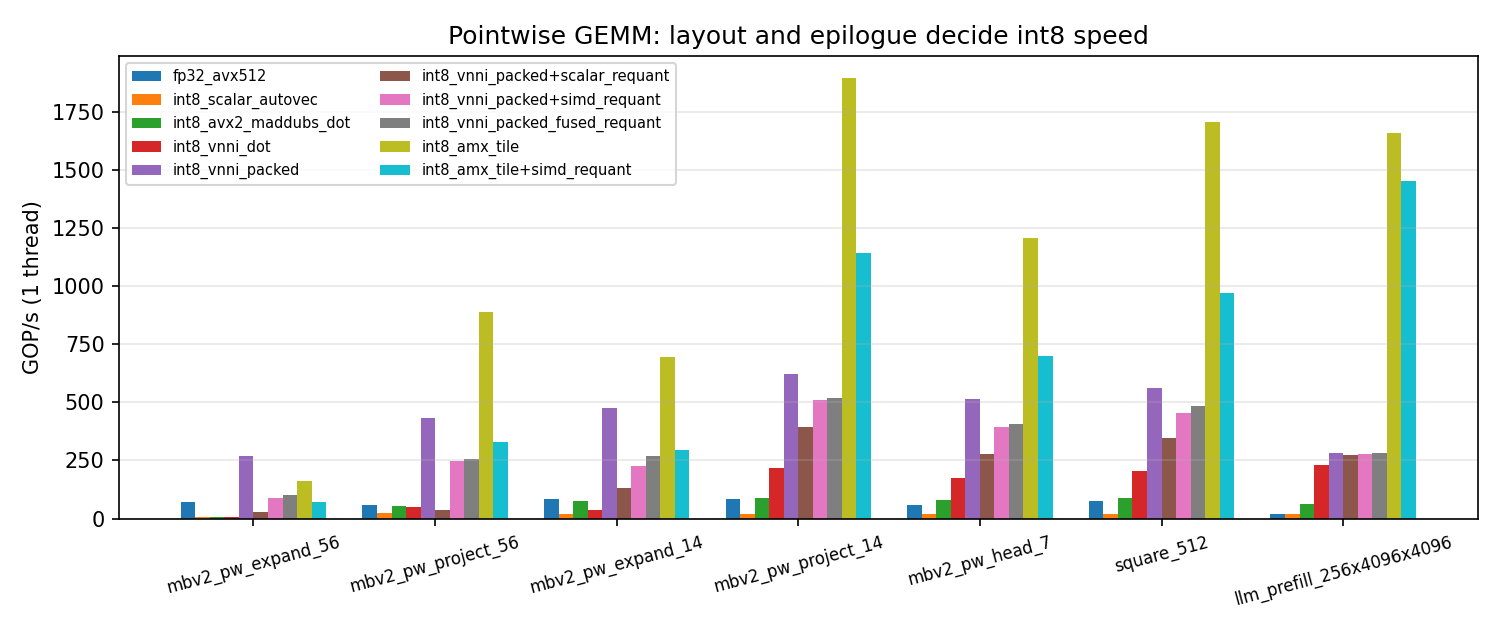
\includegraphics[width=\linewidth]{xeon8470q/gemm_bench.png}
\caption{Xeon 8470Q 1 线程 GEMM 吞吐。与 \cref{fig:gemm} 相比多了两根柱：AMX tile（黄绿）与 AMX + SIMD requant（青），以及最右的 LLM prefill 形状。}\label{fig:xgemm}
\end{figure}

\begin{table}[H]
\centering\small
\caption{Xeon 8470Q 1 线程 GOP/s（\texttt{xeon8470q/summary.json}），全部输出与参考逐位相等}\label{tab:xgemm}
\footnotesize\setlength{\tabcolsep}{3.5pt}
\begin{tabular}{lrrrrrrr}
\toprule
形状 & fp32 & 标量 & VNNI 点积 & VNNI 打包 & 打包 + 融合 rq & \textbf{AMX tile} & AMX + SIMD rq \\
\midrule
pw\_expand\_56（$K$=24） & 71.2 & 8.5 & 6.9 & 270.2 & 102.3 & 162.4 & 72.3 \\
pw\_project\_56（$K$=144） & 60.4 & 22.3 & 50.8 & 431.7 & 254.5 & 887.6 & 330.8 \\
pw\_expand\_14（$K$=96） & 85.3 & 19.6 & 35.5 & 476.9 & 268.3 & 693.7 & 296.0 \\
pw\_project\_14（$K$=576） & 82.3 & 20.2 & 215.4 & 621.7 & 519.3 & 1894.6 & 1140.5 \\
pw\_head\_7（$K$=320） & 56.6 & 20.0 & 172.5 & 514.0 & 405.4 & 1208.2 & 701.0 \\
square\_512 & 75.2 & 20.0 & 205.5 & 562.8 & 483.1 & 1703.6 & 968.9 \\
llm\_prefill $256\times4096^2$ & 18.4 & 19.9 & 230.2 & 280.1 & 280.3 & 1658.7 & 1453.1 \\
\bottomrule
\end{tabular}
\end{table}

\Cref{fig:xgemm} 的形状和 \cref{fig:gemm} 很像——打包仍然远高于逐点积、融合仍然高于标量 epilogue——但多出来的黄绿柱（AMX）在大 $K$ 的形状上把其余柱压成了矮条；
唯独最左的 pw\_expand\_56，AMX（162）比紫色的 VNNI 打包（270）还低。几处要点：

\begin{itemize}
  \item \textbf{AMX 的收益 $\propto$ $K$ 的填充率。} AMX / VNNI 打包：$K=24$ 0.60 倍、$K=96$ 1.45 倍、$K=144$ 2.06 倍、$K=320$ 2.35 倍、$K=512$ 3.03 倍、$K=576$ 3.05 倍。
        $K=24$ 时按 \cref{eq:fill} 只有 37.5\% 的乘加作用在真实数据上，62.5\% 在补零。
  \item \textbf{峰值利用率。} 按每核每周期 2048 次 int8 运算、2.1 GHz 基频估算单核 AMX 峰值约 4.3 TOP/s，1.9 TOP/s（$K=576$）是其 44\%：
        $2\times2$ 块每次只复用 A / B 各 2 次，tile load 仍占不少时间。VNNI 打包在 square\_512 上 563 GOP/s，是服务器 1 线程实测 int8 峰值 617 的 91\%，
        比本机的 56\% 高得多（\cref{sec:host}）。
  \item \textbf{prefill 形状上 VNNI 打包只有 280。} 它的外层循环每 4 行 A 就把整个 B（$4096\times4096$ = 16 MiB，超出 2 MiB L2）扫一遍，共 64 遍，B 一直从 L3 流入；
        AMX 每 32 行扫一遍 B，只有 8 遍，于是同一形状上快 5.9 倍。两者都没有 K / N 方向的 cache 分块——这正是 oneDNN 类库要做的下一步。
        fp32 版本 64 MiB 的权重连 L3 也装不下一半，跌到 18 GFLOP/s；AMX 对 fp32 是 90 倍，这个数字说的是 fp32 基线有多糟，不是 AMX 有多快。
  \item \textbf{标量循环只有 20 GOP/s。} 本机 GCC 13 是 100：汇编计数显示 GCC 13 多出 18 条 \texttt{vpdpbusd}，把标量点积自动识别成了 VNNI；GCC 11 只能先把字节扩成 16 位。
\end{itemize}

\begin{figure}[H]
\centering
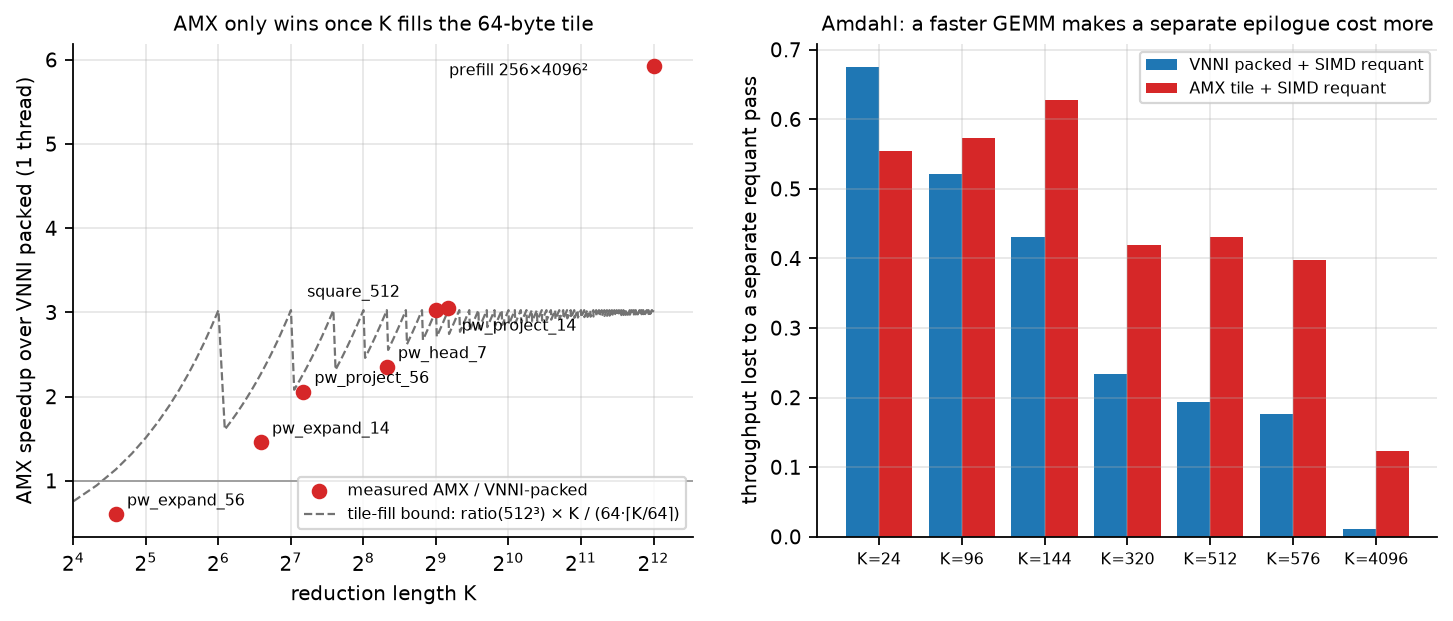
\includegraphics[width=\linewidth]{xeon8470q/amx_vs_k.png}
\caption{Xeon 8470Q。左：AMX 对 VNNI 打包的加速比随归约长度 $K$（对数轴），虚线是只考虑“$K$ 向上补齐到 64 的倍数”的上界 $\mathrm{ratio}(512^3)\cdot K/(64\lceil K/64\rceil)$；
右：单独一遍 SIMD requant 造成的吞吐损失，蓝色为 VNNI 打包、红色为 AMX tile。}\label{fig:amxk}
\end{figure}

\Cref{fig:amxk} 左图的虚线按 $512^3$ 的实测比值 3.03 缩放 \cref{eq:fill}：$K$ 刚过 64 的整数倍时补零浪费最大，曲线跳水，形成锯齿；$K\ge 512$ 后锯齿收窄到 3 附近。
实测点都在上界之下或附近：square\_512 与 pw\_project\_14 贴住上界，pw\_project\_56（$K=144$，$\eta=75\%$）2.06 低于上界 2.27，
pw\_expand\_14（$K=96$）1.45 明显低于同为 $\eta=75\%$ 的上界 2.27，pw\_expand\_56（$K=24$）0.60 落到了 1 以下——\emph{对小通道数的端侧模型，AMX 路径必须按层回退到 VNNI}。
小 $K$ 的点还低于上界，说明除了补零，每个输出块的 tile 配置、清零、store 与 spill 这些固定成本也在 $K$ 小时占比更大。
prefill 点（5.9）远高于上界，因为那里的差距来自 B 的重复流入次数，已不是 tile 填充问题。

右图读的是 Amdahl（\cref{eq:amdahl}）。蓝柱（VNNI + SIMD requant）随 $K$ 增大单调下降：$K=24$ 损失 67\%，$K=576$ 18\%，$K=4096$ 只有 1\%——GEMM 变重，requant 被摊薄。
红柱（AMX + SIMD requant）在 $K=144$--576 维持在 40--63\%，在 $K=320$ 以上明显高于蓝柱：requant 的时间不变，GEMM 却快了 2--3 倍。
以 square\_512 为例（$2\cdot512^3$ 次运算），由 \cref{tab:xgemm} 反推：VNNI 打包 GEMM 477 $\mu$s、requant 114 $\mu$s；AMX GEMM 158 $\mu$s、requant 119 $\mu$s。
requant 那一遍的绝对时间几乎不变，份额从 19\% 涨到 43\%。本机同一形状 GEMM 1267 $\mu$s、requant 177 $\mu$s，只损失 12\%。

\begin{findingbox}[：AMX 是按层选择的路径，requant 必须跟着融合]
AMX 在 $K$ 填满 64 字节 tile 时对 VNNI 打包快 3.0 倍（$512^3$），在大 prefill 形状上因为 B 少流 8 倍而快 5.9 倍；但 MobileNetV2 的 $K=24$ 层被补零到 64 后只有 0.6 倍。
GEMM 变快后，单独一遍 SIMD requant 在 $512^3$ 上从 1704 拖到 969 GOP/s（$-43\%$）。要保住 AMX 的收益，requant 必须融合进 tile store 之后的寄存器阶段，
而不是再扫一遍 int32 累加器——本实验的 AMX 路径还没有这样做。
\end{findingbox}

\begin{figure}[H]
\centering
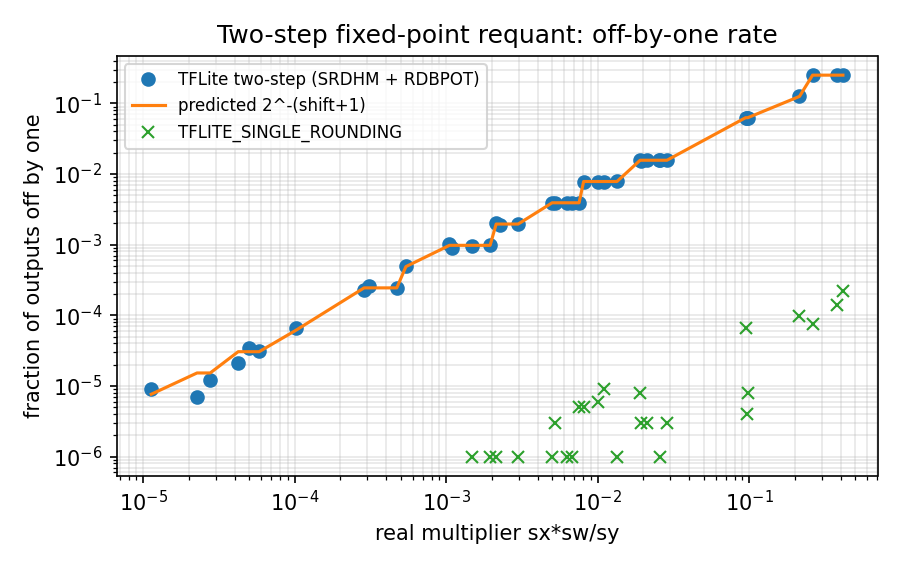
\includegraphics[width=0.82\linewidth]{xeon8470q/double_rounding.png}
\caption{Xeon 8470Q：两步定点 requant 的不一致率，坐标与图例同 \cref{fig:double}。}\label{fig:xdouble}
\end{figure}

\Cref{fig:xdouble} 与 \cref{fig:double} 肉眼无法区分：两份 \texttt{double\_rounding.csv} 的 40 行 shift、预测、两步定点、单步定点四列逐项相同，只有乘数 $m$ 的
最后一位十进制打印有差别。这是意料之中的：实验用固定种子的 NumPy 随机数和纯整数运算，与 CPU、操作系统、编译器无关。
它也是一个有用的对照——如果这张图在另一台机器上变了，问题出在实现，而不是硬件。

\begin{iqbox}{有了 AMX，为什么 oneDNN 仍然保留 VNNI 路径？}
因为 AMX 的收益依赖形状。tile 在 $K$ 方向固定 64 字节、$M$ 方向 16 行：小 $K$（MobileNet 的 1$\times$1 层 $K=24$）补零浪费 62.5\%，实测只有 VNNI 打包的 0.6 倍；
小 $M$（batch 1 的 GEMV，$M=1$）浪费 15/16 的行。另外进程要先向内核申请 XTILEDATA 状态，上下文切换要多保存 8 KB 的 tile 寄存器，对小算子这些固定成本不可忽略。
所以库按形状选路径：大 GEMM（prefill、大 batch）走 AMX，decode 的 GEMV 和小通道卷积走 VNNI / AVX-512。
\end{iqbox}

\section{本机与服务器对照}\label{sec:host}

\begin{table}[H]
\centering\small
\caption{同一份代码两台机器的比值（服务器 / 本机，1 线程），由 \cref{tab:gemm,tab:xgemm} 计算}\label{tab:cross}
\begin{tabular}{lrrrr}
\toprule
形状 & VNNI 打包 & fp32 & 标量 & 打包 + 融合 rq \\
\midrule
pw\_expand\_56 & 2.09 & 2.11 & 1.14 & 1.55 \\
pw\_project\_56 & 2.17 & 2.13 & 0.36 & 1.88 \\
pw\_expand\_14 & 2.62 & 2.20 & 0.28 & 2.14 \\
pw\_project\_14 & 2.82 & 2.03 & 0.20 & 2.64 \\
pw\_head\_7 & 2.58 & 1.65 & 0.19 & 2.36 \\
square\_512 & 2.66 & 1.92 & 0.20 & 2.53 \\
\bottomrule
\end{tabular}
\end{table}

\begin{table}[H]
\centering\small
\caption{正确性与比率类指标：两台机器对照}\label{tab:crossok}
\begin{tabular}{lll}
\toprule
指标 & 本机 & 服务器 \\
\midrule
两步定点与 ORT 一致率最小值（普通 / 平局） & 99.93\% / 98.97\% & 99.93\% / 98.97\% \\
单步定点、float、double 与 ORT（普通数据） & 100\% & 100\% \\
C++ 与 Python 逐位一致、GEMM 逐位一致 & 是 / 是 & 是 / 是 \\
maddubs 出错比例（$|w|$=64 / 100 / 127） & 0 / 99.0\% / 100\% & 0 / 98.1\% / 100\% \\
ORT int8 加速，1 线程 & 1.39--3.08 & 1.28--3.38 \\
ORT int8 加速，4 线程 & 0.76--2.14 & 0.57--1.61 \\
SIMD requant 损失，square\_512（VNNI 打包） & 12\% & 19\% \\
\bottomrule
\end{tabular}
\end{table}

两类结论在换机器时表现完全不同：

\begin{itemize}
  \item \textbf{正确性结论逐位不变。} 8 个 requant 一致率指标两台机器的 \texttt{summary.json} 逐位相同；两步舍入曲线逐点相同；饱和阈值相同。
        它们只依赖整数算术和舍入规则，与硬件无关。
  \item \textbf{“打包远快于逐点积”“融合快于标量 epilogue”是结构性的。} 服务器上 6 个 MBv2 / 方阵形状的打包 / 逐点积 2.7--38.9 倍，融合 / 标量 requant 1.32--6.85 倍，方向与本机一致。
        VNNI 打包在服务器上快 2.1--2.8 倍，大致随 $K$ 增大而升高（$K=24$ 2.09，$K=576$ 2.82）：大 $K$ 的形状更多受 int8 单元限制，能吃到服务器更强的单核；
        小 $K$ 的形状更多受循环与访存开销限制。这是由比值的趋势推断的，没有计数器确认。
  \item \textbf{标量 int8 是唯一服务器更慢的一项（0.19--0.36 倍，$K=24$ 除外）。} 这不是硬件差异而是编译器差异：GCC 13.2 把标量点积自动向量化成 VNNI，
        GCC 11.4 不会。跨主机比值混合了硬件与编译器两个因素，“标量基线”尤其不可移植。
  \item \textbf{ORT 的结论方向不变，数值变了。} 1 线程 int8 仍快 1.28--3.38 倍，4 线程仍有比 1 更差的层（depthwise 0.57、pw\_project\_56 0.86、pw\_expand\_14 0.87），
        服务器上 4 线程的情况比本机更差：服务器 fp32 kernel 的多线程扩展更好（例如 pw\_project\_56 1 $\to$ 4 线程 2.56 倍），int8 没跟上。
  \item \textbf{epilogue 份额上升。} 服务器上 GEMM 更快，同一形状的 SIMD requant 损失从 12\% 升到 19\%（VNNI）和 43\%（AMX），是 \cref{eq:amdahl} 的直接体现。
\end{itemize}

\begin{iqbox}{开发机上测出“int8 打包 GEMM 比 fp32 快 5 倍”，部署到服务器还能这样说吗？}
不能直接这样说。比值的分子分母都会变：服务器 fp32 快 1.65--2.20 倍，VNNI 打包快 2.09--2.82 倍，标量 int8 甚至慢 5 倍（编译器不同）；还有 AMX 这条本机没有的路径。
可移植的是\emph{结构}：“打包比逐点积快”“requant 要融合”“AMX 只对大 $K$ 有效”在两台机器上都成立；不可移植的是\emph{比值}，必须在目标机器、目标编译器上重测。
\end{iqbox}

\section{面试追问}\label{sec:iq}

\begin{iqbox}{给你一层 int8 卷积的 scale 与零点，写出完整的整数计算过程。}
E4：$acc[c] = \sum_k x_q[k]\,w_q[k,c] - z_x\sum_k w_q[k,c] + b_q[c]$，第二项离线折进 int32 偏置，偏置单位是 $s_x s_w[c]$。
E5：$M[c] = s_x s_w[c]/s_y = M_0\cdot 2^{-(31+\mathrm{shift})}$；先 SRDHM（$acc\cdot M_0$ 加 $2^{30}$ 后取高 32 位），再按 2 的幂舍入右移 shift 位，加 $z_y$，clamp 到 $[0,255]$；
ReLU6 时 clamp 上界是 $6/s_y + z_y$。padding 位置的 uint8 值是 $z_x$。累加上界 $255\cdot127\cdot K$，$K<66{,}311$ 时 int32 够用。
\end{iqbox}

\begin{iqbox}{TFLite 和 ORT 跑同一个 int8 模型，输出差 1，哪个对？}
都对，契约不同。TFLite 默认两步定点舍入，ORT 用 fp32 乘法加五成双。两步舍入在第一步把值量化到 $2^{-\mathrm{shift}}$ 的网格上，制造出平局，
所以不一致率约 $2^{-(\mathrm{shift}+1)}$；本实验 6 层上两步定点与 ORT 一致 99.93--99.97\%，差异永远只有 1 级，构造平局时约 1\%。
判断方法：差 1 级且比例与 $2^{-(\mathrm{shift}+1)}$ 吻合就是契约差异；差多级或比例远超预测才是 bug。部署验收要用目标 runtime 的规则生成参考输出。
\end{iqbox}

\begin{iqbox}{x86 上写 int8 GEMM，AVX2 与 AVX-512 VNNI 的区别是什么？性能差在哪？}
指令层面：AVX2 用 \texttt{vpmaddubsw} + \texttt{vpmaddwd}，中间经过饱和 int16，要求 $|w|\le64$（$|w|=127$ 时本实验 4096 列全错）；VNNI 的 \texttt{vpdpbusd} 一条指令直接累加到 int32。
但更大的性能差在布局：同样是 \texttt{vpdpbusd}，逐点积写法每个输出要一次水平求和，打包成 $[N/16][K/4][16][4]$ 后累加器沿输出列排开，没有水平求和。
本机 $K=24$ 时两者差 30.8 倍，$K=512$ 时差 2 倍；打包 GEMM 到实测 int8 峰值的 56\%（本机）和 91\%（服务器）。
\end{iqbox}

\begin{iqbox}{能不能彻底消掉两步舍入的误差？代价是什么？}
用 64 位乘积一次舍入（\texttt{TFLITE\_SINGLE\_ROUNDING}）：普通数据上 6 层与 ORT 100\% 一致；对精确舍入只在平局方向（向 $+\infty$ 对远离零）和 $M_0$ 截断误差上有差别，
最多 $2.2\times10^{-4}$（shift 1），比两步定点低三个数量级以上。代价是每个输出一次 32$\times$32$\to$64 位乘法和 64 位移位；Cortex-M 有 \texttt{SMULL}，开销很小；
AVX-512 上 \texttt{\_mm512\_mul\_epi32} 只算偶数 lane，要奇偶各做一次，本实验的 SIMD requant 已经是这样实现的。
\end{iqbox}

\section{结论}

\begin{findingbox}[：本实验的五条结论]
\begin{enumerate}
  \item 整数累加是确定的：6 种层的 int32 累加三方逐位相同，实测 $|acc|$ 比满幅上界小 5--49 倍。
  \item 舍入规则才是不确定的来源：两步定点与 ORT 差 1 级的比例按 $2^{-(\mathrm{shift}+1)}$ 变化，单次舍入在普通数据上与 ORT 100\% 一致。
  \item SIMD 指令有自己的契约：\texttt{vpmaddubsw} 要求 $|w|\le64$，超过后静默饱和。
  \item 速度由布局与 epilogue 决定：打包比逐点积快 2.0--30.8 倍，融合 requant 比标量 epilogue 快 1.2--3.5 倍；ORT int8 在多线程、depthwise 上可能比 fp32 慢。
  \item AMX 只在 $K$ 填满 tile 时赢（$512^3$ 3.0 倍、prefill 5.9 倍、$K=24$ 0.6 倍），且 GEMM 越快，单独的 requant 越贵（$-43\%$）。
\end{enumerate}
\end{findingbox}

\subsection*{20 秒讲法}

我把 int8 推理从 int32 累加到 requant 回 uint8 完整写了一遍，和 ONNX Runtime 逐元素比对：累加逐位相同，但 TFLite 的两步定点舍入会在约 $2^{-(\mathrm{shift}+1)}$ 的输出上差 1 级，
这是契约差异，不是 bug。性能上，同一条 VNNI 指令，换成打包布局在小通道层上快 30 倍；requant 必须融合进寄存器，否则一遍 epilogue 能吃掉八成吞吐。
到有 AMX 的 Sapphire Rapids 上，大矩阵快 3--6 倍，但 MobileNet 的 $K=24$ 层补零后反而慢，所以 AMX 要按层选。

\begin{caveatbox}
\begin{itemize}
  \item 不能推出 ARM 上的结论：Cortex-A 的 \texttt{sdot} / \texttt{smmla}、Cortex-M 的 \texttt{SMLAD} 吞吐与 VNNI 完全不同，只有“布局与 epilogue 融合比指令重要”这条可以迁移。
  \item ORT 的加速比依赖 ORT 版本选的 kernel；这里只说明 int8 不保证更快，尤其是多线程和 depthwise。服务器上的 ORT 版本未单独记录。
  \item 两步舍入的不一致率是在随机输入上测的；真实模型里如果某层恰好落在平局附近，比例会更高（构造平局时 0.45--1.03\%）。
  \item GEMM 都是 1 线程、单一形状集合；打包 GEMM 只有 16 列一组的累加器分块和 4 行寄存器块，没有 cache 分块，离 oneDNN / XNNPACK 还差一截，绝对 GOP/s 不代表库的水平。
  \item 自写 fp32 GEMM 只到本机 fp32 峰值的约四分之一，“int8 对 fp32 快 5 倍”的比值被弱基线放大；公平的 int8 / fp32 对比看 ORT。
  \item 跨主机比值混合了硬件与编译器（GCC 13.2 对 11.4）两个因素；AMX 峰值 4.3 TOP/s 是按规格估算的，44\% 的利用率受这个估算影响。
  \item 没有硬件性能计数器：prefill 形状上“B 从 L3 反复流入”是由循环结构推出的，没有用计数器确认。
\end{itemize}
\end{caveatbox}

\section{复现}

\begin{lstlisting}[language=bash]
cd solutions/edge-runtime/int8-kernels
python -m pytest -q tests                                          # reference vs C++ vs ORT; requant properties
python scripts/run_experiments.py --only requant rounding saturate  # correctness, seconds
python scripts/run_experiments.py --only gemm ort                  # timing, ~20 s, idle machine

# server rerun (Xeon 8470Q, NUMA1 physical core, AMX path compiled in on Linux)
taskset -c 60 python scripts/run_experiments.py --only gemm
\end{lstlisting}

\sloppy
C++ 由 \texttt{edge\_harness.cpp.build} 按源码哈希编译到 \texttt{cpp/bin/}，三种模式：\texttt{--mode=conv}（卷积 + 四种 requant）、
\texttt{--mode=bench}（7 种 GEMM，Linux 上有 AMX 时再加 2 种）、\texttt{--mode=saturate}（饱和计数）。
原始数据在 \nolinkurl{solutions/edge-runtime/int8-kernels/artifacts/raw/}（服务器在其 \nolinkurl{xeon8470q/} 子目录），
图由 \texttt{run\_experiments.py} 从原始数据生成；服务器的 \texttt{amx\_vs\_k.png} 由仓库根目录的
\nolinkurl{scripts/plot_server.py} 从 \nolinkurl{xeon8470q/} 的原始数据生成。


\begin{thebibliography}{99}
\bibitem{jacob2018} B.~Jacob, S.~Kligys, B.~Chen, et al. Quantization and Training of Neural Networks for Efficient Integer-Arithmetic-Only Inference. \emph{CVPR}, 2018.
\bibitem{onednn} Intel. oneAPI Deep Neural Network Library (oneDNN). \url{https://github.com/uxlfoundation/oneDNN}.
\bibitem{ort} ONNX Runtime developers. ONNX Runtime. \url{https://onnxruntime.ai}.
\bibitem{roofline} S.~Williams, A.~Waterman, D.~Patterson. Roofline: An Insightful Visual Performance Model for Multicore Architectures. \emph{Communications of the ACM}, 52(4), 2009.
\end{thebibliography}

\end{document}
